\input{preamble}

\begin{document}

% \ifpdf
% \DeclareGraphicsExtensions{.pdf, .jpg, .tif}
% \else
% \DeclareGraphicsExtensions{.eps, .jpg}
% \fi

%\maketitle


%\begin{abstract}
%\end{abstract}
%-----
\centerline{\textbf{Quantum limited parametric amplifier for millimeter}}
\centerline{\textbf{and submillimeter astrophysics}}
%\section*{Introduction} %use the * if you dont want numbering
% \section*{Abstract}
% \emph{
\begin{abstract}
This proposal is to develop a technology that would significantly improve the noise performance and available instantaneous bandwidth for coherent receivers operating up to $\approx$ 1 THz, i.e (sub)millimeter wavelengths. We propose to build a Traveling-wave Kinetic Inductance Parametric Amplifier (TKIP) to provide gain before mixer down conversion. The TKIP can provide quantum limited noise performance across an octave bandwidth, which relaxes the requirements on the mixer and afterwards. Although the TKIP could be used in receivers at a variety of facilities, (e.g SOFIA, CCAT), we propose to demonstrate its capabilities in an ALMA band 3 receiver. Here, use of the TKIP would mean a factor $\approx$ 2 better noise and factor $\ge$ 5 broader instantaneous bandwidth. Such improvement in receiver performance would accelerate pursuit of and provide new access to scientific objectives at these wavelengths.
\end{abstract}
% }

\subsection*{Statement of problem}
High resolution spectroscopic observations in millimeter to submillimeter wavelengths are made using using telescopes with heterodyne receiver systems. In these receivers, power radiated from the sky is optically focused into a feed horn, then mixed to a lower intermediate frequency (IF) using an SIS mixer, then the IF signal is amplified with a low noise transistor amplifier (LNA), and then further processed and detected. There is a loss in signal power when the mixer performs the conversion to the IF frequencies. Additionally, the LNA adds noise power to the IF. A low power, i.e `faint', astrophysical signal can therefore escape detection because the conversion loss of the mixer shifts the signal power below the noise power of the LNA. This limitation on \emph{sensitivity} to faint sources is one problem to be addressed by this project.

The mixer has a certain bandwidth over which it is sensitive to signal. The lowest noise LNAs provide the required gain over a bandwith that is much narrower than the mixer bandwidth. Thus, to measure a signal over the entire mixer bandwith, it is necessary to increment the local oscillator (LO) frequency of the mixer multiple times to shift the signal into the bandwidth of the LNA. Incrementation of the LO comes at the expense of observation time. This limitation on \emph{instantaneous bandwidth} is another problem to be addressed by this project. 

\subsection*{Proposed solution}
We propose to develop an amplifier to be inserted immediately before the mixer in a heterodyne receiver setup. This amplifier would provide enough gain over the full mixer bandwidth to relax the noise performance required of the LNA, with improvement to the receiver's sensitivity. This also permits the use of an LNA that covers the full mixer bandwith.
    
Development of this new amplifier, to be called the wTKIP\footnote{Throughout this proposal,``TKIP'' refers to those devices for use at unspecified frequency bands, whereas wTKIP refers to the proposed device which is optimized for use at the W-band and $\mu$TKIP refers to the device described in \cite{Eom2012} \label{foot:TKIP}.}, would constitute a major breakthrough in the performance of heterodyne receiver systems for (sub)millimeter waves. As a specific demonstration of its impact, we propose to develop a W-band  (80 - 116 GHz) amplifier suitable for use in Atacama Large Millimeter/Submillimeter Array (ALMA) Band 3 because: one, the wTKIP would significantly improve receiver capabilities in this band and therefore has great scientific benefit; two, the group of my proposed JPL advisor has already initiated work on the wTKIP using seed funding, which is now exhausted, provided by the ALMA technology development program; and three, the ALMA team has encouraged the JPL group to apply for additional funding to demonstrate a wTKIP receiver on their array. The proposed work fits nicely between reasons two and three because it aims to develop the TKIP technology to  state where it is ready to be used in an ALMA W-band receiver. After demonstration on ALMA, the goal is to use the technology at other facilities, such as SOFIA, where a TKIP wideband receiver system would enable spectroscopic capabilities at a rate comparable with HIFI on Herschel whose cryogenic mission has now ended; and CCAT, where use of the TKIP would enable a very fast spectral line survey instrument in the atmospheric windows to complement ALMA; and other applications like coherent receiver systems for interferometry or correlation receivers to tackle difficult continuum observations such as the CMB B-mode polarization.


% because it would to develop this technology; and three, because the wTKIP would significantly improve receiver performance in this band.   
% one, the ALMA technology development program has already given some seed funding for this amplifier, which is now exhausted;


\section*{Scientific merit}
Millimeter and submillimeter wave astronomy can provide information about processes associated with clouds of dust and molecular gas, such as star formation. Progress toward understanding these processes is in accordance with the scientific priorities declared in the National Academies 2010 decadal survey\footnote{See decadal survey chapter 2 on ``the compelling questions for the next decade and beyond'' with regard to ``origins''.} as well as NASA’s overall scientific goals\footnote{See science goals listed in section 4.4 of the 2014 NASA Science Plan.}. In general, the proposed research will result in vastly improved observing performance and efficiency for accomplishing these priorties. 
%provide new technology that significantly enhances the speed and scientific reach available to address these priorities. Here are a few specific examples particular to ALMA's W-band.
%Millimeter and submillimeter wave astronomy is undergoing a transition from continuum surveys/number counts and detailed studies of single objects to large spectroscopic surveys designed to systematically explore the properties of astronomical environments. 

\paragraph*{Molecular Gas and dust emission and absorption in submillimeter galaxies}
Submillimeter galaxies (SMGs) trace a large fraction of the star formation activity in the universe and are dominated by objects undergoing rapid star formation at relatively high redshifts (1 $<$ z $<$ 3). ALMA can locate SMGs precisely and obtain a redshift using sequential observations with different local oscillator tunings to cover an entire ALMA band to detected one or more redshifted CO lines. Currently, covering the whole of ALMA band 3 requires setting the local oscillator (LO) to 5 different frequencies. An increase in instantaneous bandwidth to cover the entire band combined with a reduction in system temperature would allow detection of one or more CO lines at all redshifts in a single LO tuning and provide an increase in continuum sensitivity that would enable at least an order of magnitude increase in the speed of imaging and spectroscopy of high redshift SMGs.

\paragraph*{Galaxy clusters}
The Sunyaev-Zel’dovich (SZ) effect is a distortion of the cosmic microwave background (CMB) spectrum caused by the scattering of CMB photons as they pass through the hot intracluster medium (ICM) of massive galaxy clusters. The brightness of the spectral distortion is independent of redshift and the SZ signal strength  serves as an excellent proxy for cluster mass. These characteristics make the SZ effect a useful window into the astrophysical processes that shape galaxy clusters. Wide-field high angular resolution imaging with moderate spectral resolution in bands from \SIrange{15}{300}{GHz} would allow unprecedented determination of the cluster gas temperature and density profiles and therefore the cluster mass and dynamics especially when combined with Xray data from e-Rosita and optical weak lensing surveys. These measurements could only be made with a significant increase in sensitivity, frequency coverage and mapping speed over the
existing single dish and interferometric instruments.

\paragraph*{Star formation in the milky way}
Star formation in the Milky Way takes place in molecular clouds that are of high enough density. Understanding how molecular clouds of low density transition to clouds with density high enough to support star formation and why such a small fraction why such a small fraction of the cloud mass is contained in dense gas is key to determining the dominant physical processes that control the star formation rate. 

  \begin{wrapfigure}{L}{0.42\textwidth}
    \vspace{-20pt}
  	  \centering
    \begin{tabular}{ll}
    \toprule
    Atmospheric window  & \SI{100}{GHz}  \\
    \midrule
    Opacity & 0.02 \\
    T$_\text{sys}$ for T$_\text{rec}$ = 5 $\frac{h \nu}{k_B}$ & \SI{30}{\kelvin} \\
    T$_\text{sys}$ for T$_\text{rec}$ = 1.5 $\frac{h \nu}{k_B}$ & \SI{11.3}{\kelvin} \\
	Integration time reduction & $\times$3.9 \\
    % \midrule
%     Opacity for 1.3 mm PWV& 0.04 \\
%     T_{sys} for T_{rec} = 5 $\frac{h \nu}{k_B}$ & 36 \\
%     T_{sys} for T_{rec} = 2 $\frac{h \nu}{k_B}$ & 21 \\
%	  ratio of integration time & 3.0 \\
    \bottomrule
    \end{tabular}%


     \vspace{-10pt}
  \caption{Expected performance improvement for TKIP assuming identical instantaneous receiver bandwidths in the \SI{100}{GHz} atmospheric window. The opacity assume \SI{0.66}{\mm} precipitable water vapor, commensurate with a site like Cerro Chajnantor. 5 $\frac{h \nu}{k_B}$ represents the current best receivers and 1.5 $\frac{h \nu}{k_B}$ is the expectation for the wTKIP.}
      \vspace{-15pt}
  \label{tab:ALMA_wTKIP}%
   \end{wrapfigure}
Spectral lines from different molecular transitions probe different volume densities and temperatures, and time-dependent chemistry favors the production of different molecules at distinct times. With 34 GHz of instantaneous bandwidth, a receiver based on this technology would have the ability to observe multiple molecular transitions simultaneously and probe these different regions. With suitable back end processing power, this spectral multiplex advantage would decrease observing time by the number of lines simultaneously observed, modulo integration time differences due to varying line strengths. Such back end processing bandwith is achievable at low price using a bank of 12 CASPER ROACH2 spectrometer boards \cite{ROACHweb}, for example. 


% Frontier science at these wavelengths is contained in the signals that are faint. This creates a justification to minimize instrument imposed limitations on sensitivity.
%
% from SAFIRE
%  ``imaging these regions in lines arising from molecular, atomic and ionized components, along with the dust emission. These observations are critical to achieving a clear understanding of the process which result in the formation of stars, and which control star formation on a galactic scale in starburst galaxies''
%
 
\section*{Technical merit}
General figures of technical merit of the TKIP include the following:

\begin{itemize}
\item Currently state-of-the-art  SIS mixers and IF amplifiers limit instantaneous receiver bandwith $\le$ 10 GHz. Use of a TKIP as a front end amplifier would permit the use of lower gain, wider bandwidth mixers and IF amplifiers in the receiver signal path.  Not only would it be easier to approach the quantum limit (QL) with such a receiver, but the IF bandwidth could be widened, we believe, by over an order of magnitude, increasing the speed for line surveys by the same factor and greatly improving the sensitivity for continuum observations.

\item The TKIP is significantly more sensitive than transistor amplifiers. Theoretically, the TKIP should reach the standard quantum limit (T$_\text{noise} k_B$ = $\sfrac{1}{2}$ photons per second per Hz). Transistor amplifiers at best add noise about five times higher than this limit.

\item Superconducting paramps using Josephson junctions operate at the QL, but these are narrow band devices with fractional bandwidth of at most only a few percent due to the use of resonant circuits. The TKIP has a bandwidth approaching that of transistor amplifiers, with octave bandwidth being readily achievable.

\item Other superconducting paramps have operated at tens of GHz and transistor amplifiers operate with reduced fractional bandwidth up to a few hundreds of GHz. Owing to its simple distributed design, the TKIP will potentially operate up to the gap frequency of its superconducting material; that is,  $\lesssim$ \SI{1.4}{THz} or $\gtrsim$ \SI{214}{\micro \meter} for NbTiN.

\item Compared to transistor amplifiers, the TKIP requires lower temperature operation, around \SIrange{1}{4}{\kelvin} (Fig.~\ref{Fig:W-Band_Expected_Gain_Noise}b). However, one, commercially available pulse tube coolers easily reach that temperature; and two, when the TKIP replaces an SIS mixer, the TKIP can reuse the existing cryogenic infrastructure put in place for the SIS mixer.
\end{itemize}

For the particular application of the wTKIP on ALMA band 3,  Tab.~\ref{tab:ALMA_wTKIP} summarizes the expected performance improvements. In addition to the shortened integration times, observations are also expedited by elimination of the need to increment the LO to image the entire band. This means simultaneous detection of spectral lines, simplified spectral index measurements, etc.




\section*{Technology description}
The TKIP, Fig.~\ref{Fig:muTKIP}a,  consists of an electrically long section of superconducting transmission line,  in coplanar waveguide (CPW) format. An intense ``pump'' waveform at angular frequency $\omega_P$, and a weak ``signal'' waveform at frequency $\omega_S$ are guided into one end of the transmission line. Power is transferred from the pump waveform to the signal waveform as the two travel along the line. The signal emerges amplified at the other end of the line, and the pump in correspondingly attenuated.  

  \begin{figure}
      \vspace{-20pt}
      \begin{center}
	     \begin{tabular}{cc}
\begin{overpic}[width=0.55\textwidth]{images/TKIP.png}
	\put (90,50) {\textcolor{black}{\LARGE \textbf{a}}}\end{overpic}
 &
% \multicolumn{2}{c}{
\begin{overpic}[width=0.40\textwidth]{images/Stop_Bands.png}
\put (90,68) {\textcolor{black}{\LARGE \textbf{b}}}\end{overpic}%}
\\
	     \end{tabular}
      \end{center}
      %\vspace{-20pt}
	  \caption{\textbf{a}, A picture of the microwave band TKIP, ($\mu$TKIP), which consists of a 0.8 m length of NbTiN CPW line arranged in a double spiral to reduce resonances due to coupling between adjacent lines. The line is periodically loaded by widening a short section after every length D=877 micron as shown on the right, producing the stop band and dispersion characteristics. The phase velocity on the line is 0.1c due to its large kinetic inductance. \textbf{b}, An illustration of the effect of the periodic loading pattern (shown schematically) on the transmission of an infinite transmission line. The gray regions represent stop bands; waves in these frequency ranges decay evanescently. As the fractional width of the third stop band is much larger than the first, the pump can be placed at a propagating frequency while $3\omega_P$ is blocked.}
      \vspace{-10pt}
    \label{Fig:muTKIP}
   \end{figure}

% \begin{wrapfigure}{L}{0.65\textwidth}
%   %\vspace{-20pt}
%   %\begin{center}
% 	  \centering
%      \begin{tabular}{cc}
% \begin{overpic}[width=0.3\textwidth]{images/Phase_Response.png}
% \put (93,70) {\textcolor{black}{\LARGE \textbf{a}}}\end{overpic}
% &
% \begin{overpic}[width=0.3\textwidth]{images/Stop_Bands.png}
% \put (90,70) {\textcolor{black}{\LARGE \textbf{c}}}\end{overpic}
% \\
% \multicolumn{2}{c}{
% \begin{overpic}[width=.6\textwidth]{images/TKIP.png}
% \put (95,40) {\textcolor{black}{\LARGE \textbf{b}}}\end{overpic}}
% \\
%      \end{tabular}
%   %\end{center}
%       %\vspace{-20pt}
%  \caption{1 Phase response to DC current and amplifier design.
% Top left, This plot illustrates the nonlinearity of the kinetic
% inductance. A NbTiN coplanar waveguide (CPW) transmission
% line was measured in transmission using a microwave network
% analyzer. Using bias tees, a DC current was passed down the
% center conductor. The resulting microwave phase shift (measured
% at 4 GHz) displays a quadratic dependence with current.
% As an illustration of this effect, we can pass a d.c. current down the center conductor of the CPW transmission line while we apply the signal waveform and measure the phase shift, $\Delta \theta \approx \beta \ell$, of the signal waveform. $\beta = 2\pi f_P \sqrt{\overbar{L}(I)\overbar{C}}$ depends on the current current and $\ell$ is the length of the line. In the case of the TKIP, the a.c. current due to the pump is responsible for the phase shift.
%  Bottom,
% A picture of the TKIP (left) which consists of a 0.8 m length of
% NbTiN CPW line arranged in a double spiral to reduce resonances
% due to coupling between adjacent lines. The line is periodically
% loaded by widening a short section after every length D=877
% micron as shown on the right, producing the stop band and
% dispersion characteristics. The phase velocity on the line is 0.1c
% due to its large kinetic inductance. Top right, An illustration of the
% effect of the periodic loading pattern (shown schematically) on the
% transmission of an infinite transmission line. The gray regions
% represent stop bands; waves in these frequency ranges decay
% evanescently. As the fractional width of the third stop band is
% much larger than the first, the pump can be placed at a propagating
% frequency while $3\omega_P$ is blocked.}
%       \vspace{-10pt}
%     \label{Fig:muTKIP}
%    \end{wrapfigure}
The TKIP exploits the natural nonlinear behaviour of the surface inductance of the superconductor.  The surface inductance (``kinetic inductance'') is due to the kinetic energy of the supercurrent. The series inductance per unit length, $\overbar{L}$, of the transmission line depends on the current, $I$, as $\overbar{L}(I) = \overbar{L}(0)[1+ \sfrac{I}{I_*}^2]$, where $I_*$ sets the scale of the effect. 

The current on the transmission line due to the intense pump waveform makes the inductance of the line vary periodically. Thus, the non-linear inductance is the parameter that is used to generate the amplification (``parametric amplifier'').  For the superconductors used, the nonlinearity is almost purely reactive meaning that these devices are non-dissipative. Consequently, one, the TKIP should not dissipate power, and two, the TKIP need not produce thermal noise or shot noise and, in principle, the noise performance is limited only by quantum mechanics.


\subsection*{Theory of operation}
The phase velocity depends on inductance, $v_{p}(I)= \sfrac{1}{\sqrt{\overbar{L}(I)\overbar{C}}} \approx v_{p}(0)(1 - \alpha I^2 / 2 I^2_*)$, where $\alpha$ is a measure of the kinetic inductance. This is analogous to the optical Kerr effect where the refractive index is intensity dependent. The intensity dependence of the refractive index results in the nonlinear process of four-wave mixing (FWM). Fiber optic paramaps, which operate at optical/near-IR frequencies, are based on this mixing \cite{Hansryd2002} and coupled mode equations have been developed to quantify their parametric gain. We can use this theory \cite{Stolen1982} to predict the gain of the TKIP. 

 
The FWM allows for two different  pump waveforms, but we consider the degenerate case where the two are equal. When the pump and the signal are allowed to mix, an ``idler''  waveform is  generated. The relationship between the frequencies of the three waveforms is by $\omega_S+\omega_I = 2\omega_P$ or $\omega_S+\omega_I = \omega_P$, where $\omega_I$ is the idler waveform angular frequency.


According this theory \cite{Stolen1982} the gain of a weak signal in the presence of a strong pump can be written as,
\begin{equation}
	G_S = 1+ \left[ \frac{\gamma P_P}{g} \sinh g \ell \right]^2.
\end{equation}
Here $\ell$ is the length of the transmission line, $P_P$ is the pump power, and $\gamma$ is a measure of the nonlinearity such that $\Delta \theta = \gamma P_P \ell$ is the power-dependent phase shift, in radians, resulting from the intensity dependent index. The parameter $g$ depends on dispersion $\Delta \beta$,
\begin{equation}
	g^2 = - \Delta \beta \left[ \frac{\Delta \beta}{4} + \gamma P_P\right].
\end{equation}
and the dispersion in turn depends on the values of the propagation constant $\beta(\omega)$ at the signal, idler and pump frequencies through $\Delta \beta = \beta(\omega_S) + \beta(\omega_I) -2\beta(\omega_P)$.


To a good approximation, a superconducting CPW transmission line is dispersionless, $\Delta \beta = \gamma = 0$. Thus the parametric gain in the signal is a quadratic function of the non-linear phase shift, $G_S = 1 + (\Delta \theta)^2$, since  $ \lim_{g \to 0} \frac{\gamma P_P}{g} \sinh g \ell =  \gamma P_P \ell = \Delta \theta$.

  
For a dispersive transmission line, $\Delta \beta \, , g \neq 0 $ and the presence of the $\sinh  g \ell$ term in the gain
expression can result in exponential gain. Maximum gain occurs when $\Delta \beta = -2 \gamma P_P$ and $\ell$  is long enough so that $\Delta \theta \gg 1$. The gain is then $G_S \approx \sfrac{e^{2\gamma P_P \ell}}{4} = \sfrac{e^{2\Delta \theta}}{4}$. Fiber optic paramps are able to access the exponential gain regime, producing gain $>$ 60 dB, because they have builtin dispersion.  

Dispersionless nonlinear media, such as our superconducting transmission line, support efficient harmonic generation. The formation of pump harmonics would severely limit the gain of the TKIP \cite{Landauer1960}. We therefore take the approach of introducing  dispersion into  the TKIP by periodically loading the line, Fig.~\ref{Fig:muTKIP}b. The spacing between the loads is chosen to place a stop band around $3\omega_P$, the frequency of the lowest pump harmonic. Additionally, the loads are slightly offset to introduce dispersion features around the pump frequency itself, $\omega_P$. This allows us to access the exponential gain regime. Thus, engineering dispersion simultaneously solves the problem of harmonic generation and provides access to the exponential gain regime.   


\section*{Previous work}
Non-linear response in electronic circuits has long been used to obtain parametric amplification. In the 1950s, for example, low-loss varactor diodes with voltage-variable capacitance allowed the construction of amplifiers operating in the microwave to millimeter-wave bands \cite{Nergaard1959}.  The nonlinear inductance of Josephson junctions in superconducting circuits can represent a nearly ideal nonlinear reactance, which led to strong interest in the development of Josephson-junction amplifiers \cites{Russer1969, Feldman1975}, and by the late 1980s improved junction fabrication techniques allowed sophisticated devices to be produced reliably, and narrow-band microwave amplifiers with excellent noise performance approaching the quantum limit were demonstrated \cites{Smith1985,Yurke1988, Movshovich1990}. 


  \begin{wrapfigure}{R}{0.75\textwidth}
      \vspace{-20pt}
      \begin{center}
	     \begin{tabular}{cc}
\begin{overpic}[width=0.37\textwidth]{images/Gain_Curve.png}
	\put (93,70) {\textcolor{black}{\LARGE \textbf{a}}}\end{overpic}
 &
\begin{overpic}[width=0.37\textwidth]{images/Gain_Variation.png}
\put (85,70) {\textcolor{black}{\LARGE \textbf{b}}}\end{overpic}
\\
	     \end{tabular}
      \end{center}
      %\vspace{-20pt}
	  \caption{\textbf{a}, Measured gain of a $\mu$TKIP using a 0.8 m NbTiN CPW (gray line). The measured gain is smoothed over 40 MHz to produce the blue line. \textbf{b}, Detail of gain curve between 6.6 and 7.1 GHz. The rapid gain variations are due to reflections at the ends of the device. We expect to reduce these reflections through better impedance matching and by implementing ground ties to connect the CPW grounds.}
      \vspace{-10pt}
    \label{Fig:TKIP_Gain}
   \end{wrapfigure}
A drawback of early implementations of Josephson paramps was that the amplification was only achieved over a narrow bandwidth. Tuned circuits used to enhance the effect of nonlinearity produced intrinsically narrow-band devices, unsuitable for applications needing wide instantaneous bandwidth. An alternative design \cites{Tien1958,Tien1961, Cullen1958, Sweeny1985}  dispensed with the resonant circuit and the device took the form of a nonlinear transmission line with either a distributed nonlinearity or a series of discrete nonlinear elements. Though intrinsically wide band, it did not result in practical devices because of dispersive effects and problems associated with producing the required degree of nonlinearity.   
   
The research group of my proposed JPL advisor constructed a TKIP with significant gain in the microwave frequency band 9.5 - 13.5 GHz ($\mu$TKIP). The success of this  device was due to the use of  NbTiN superconductor, which exhibits strong nonlinearity and low loss. The group reported its breakthrough in the journal Nature Physics \cite{Eom2012}. The publication makes clear what improvements need to be made in order to realize the full potential on this new technology. They include, one, increasing the  gain and eliminating a fine-scale variation of the gain; two, understanding and suppressing noise in excess of the QL. The group has made progress toward these improvements and the proposed  project will continue their work.  Presently, the group has designed and fabricated a first iteration of a W-band TKIP (wTKIP) using, in part, seed funds from an NRAO ALMA technology development grant, but these funds were exhausted before testing could commence. 


% \section*{expected results}
% \subsection*{Amplifier specification}
% TKIP works up to the gap frequency (>1 THz for NbTiN),
%
% \section*{Methodology}
% \subsection*{Timeline}
%
% \section*{Techniques}
% \emph{explanation of new or unusual techniques}
%
% Use travel traveling wave amplifier design


\section*{Approach}
\subsection*{Construction of Test Setup for W-Band Paramp}
I propose to construct a test setup capable of measuring the gain and noise of the prototype W-band TKIP (wTKIP). The noise measurement would be done via the Y-factor method, which uses a variable temperature termination. This will involve installing waveguides in a cryostat with a 1 K cryocooler and a cryogenic HEMT amplifier. To avoid saturation, the ability to null the pump tone before it enters the HEMT, will be built into the system. An existing lab down converter system will be used to shift the output band to a range that can be measured by a microwave spectrum analyzer.


\subsection*{Amplifier Development}
The performance of the wTKIP will be measured and improvements to its design will be made.  Gain ripple observed in the wTKIP will be addressed by implementing ground plane straps and improved couplings to the device, including better matching for in-band signal and dissipation of out of band signals.  Excess noise will be suppressed by improved heat sinking. 

\paragraph*{Test wTKIP}
The wTKIP uses the same CPW geometry as the $\mu$TKIP (\cite{Eom2012}), but the periodic structure has been adjusted for a pump at \SI{118}{GHz}. The overall length of the transmission line is decreased, but the length measured in wavelengths is somewhat increased as the operating frequency is ten times higher. Fig.~\ref{Fig:W-Band_Expected_Gain_Noise}a shows the calculated gain based on the coupled mode theory, assuming a pump power, $P_P$, half of that used for the microwave device.
  % \begin{wrapfigure}{L}{0.5\textwidth}
  %     \vspace{-20pt}
  %     \begin{center}
  % 	     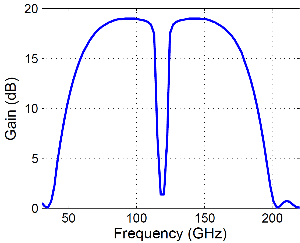
\includegraphics[width=0.48\textwidth]{images/W-Band_Expected_Gain.png}
  %     \end{center}
  %     \vspace{-20pt}
  % 	  \caption{Calculated gain of the W-band TKIP, assuming a pump power half as large as what was used with the microwave TKIP described in \cite{Eom2012}. The dip in the center is dueto dispersion around the pump frequency.}
  %     \vspace{-10pt}
  %   \label{Fig:W-Band_Expected_Gain}
  %  \end{wrapfigure}
  \begin{figure}
      \vspace{-20pt}
      \begin{center}
	     \begin{tabular}{cc}
\begin{overpic}[width=0.48\textwidth]{images/W-Band_Expected_Gain.png}
	\put (90,68) {\textcolor{black}{\LARGE \textbf{a}}}\end{overpic}
 &
% \multicolumn{2}{c}{
\begin{overpic}[width=0.53\textwidth]{images/Noise_Transmission_vs_Temp_wTKIP.png}
\put (90,60) {\textcolor{black}{\LARGE \textbf{b}}}\end{overpic}%}
\\
	     \end{tabular}
      \end{center}
      %\vspace{-20pt}
	  \caption{\textbf{a}, Calculated gain of the W-band TKIP (wTKIP), assuming a pump power half as large as what was used with the microwave TKIP described in \cite{Eom2012} ($\mu$TKIP). The dip in the center is due to dispersion around the pump frequency. \textbf{b}, Calculated transmission through a $100\lambda$ section of the NbTiN line versus temperature in blue. The green line shows the estimated noise contribution of the device, assuming no non-thermal noise sources.}
      \vspace{-10pt}
    \label{Fig:W-Band_Expected_Gain_Noise}
   \end{figure}  
  
  
We will determine the sensitivity (noise), gain characterists of the first generation wTKIPs and make necessary design corrections to enhance their performance.   

\paragraph*{Ground plane straps}
A typical gain curve is shown in Fig.~\ref{Fig:TKIP_Gain}. While the average gain displays a broad maximum, reaching 20 dB, there is a fine-scale variation of the gain due to standing waves created by reflections at the ends of the line.  These ripples were more severe in earlier $\mu$TKIP and have been reduced through better impedance matching. A further improvement would be to connect the CPW ground planes with “straps” to prevent the excitation of a slot line mode on the CPW. Design and implementation of straps and other impedance controls on the wTKIP will be an objective for this project.  


\paragraph*{Supression of excess noise}
Since their publication \cite{Eom2012}, the JPL group determined that the excess noise in their $\mu$TKIP, approximately 3 or 4 photons in excess to the quantum limit of $\sfrac{1}{2}$ photon (per second per Hz bandwidth), was thermal in origin. They came to this conclusion by measuring the noise of the $\mu$TKIP while pulsing the pump waveform with on-time ranging from 0 to 100 percent.  They found that the excess noise decreases as the on-time decreases. Further, they found that the temperature of the $\mu$TKIP chip increases with pump power. These observations indicate that the amplifier is not operating in a completely dissipationless mode and that at least a component of the observed excess noise is thermal noise. Fortunately, at 100 GHz, we expect that the wTKIP can still be essentially quantum limited at cryocooler temperatures Fig.~\ref{Fig:W-Band_Expected_Gain_Noise}b, but the chip must be prevented from significantly heating. A goal of this project will be to study the effect of better heat sinking on the excess noise of the wTKIP.


\paragraph*{Improved coupling to device} For the first iteration wTKIP, we will use commercial waveguide to WR10 transitions and WR10 sparkplug connectors to bring the millimeter-wave power into and out of the device housing. The power is brought onto the chip using wire bonds. While these devices will be sufficient for initial testing, reflections are likely to be a limitation. Further iterations of the wTKIP will include on-chip waveguide probes and reflectionless filters.


\subparagraph*{Waveguide probes:} To reduce gain ripple and improve performance, it will be necessary to improve signal coupling into and out of the paramp. Full band waveguide probes coupled to transmission lines have been developed for use up to THz frequencies. An example of a simple design is the radial probe \cite{Withington1996} which has a feed impedance of approximately 20 Ohms. The Microdevices Lab at JPL has previously manufactured similar probes for SIS mixer based instruments (e.g. \cite{Kooi2003}). The impedance of the TKIP CPW transmission line is typically 50 Ohms or larger so coupling to these probes requires an impedance matching section which potentially limits the bandwidth. As used in the MUSIC \cite{Golwala2012} array, another option for the TKIP is to couple incoming radiation through a set of multiple long slot antennas which are combined in a phased array. This potentially gives wide bandwidth and the feed impedance of the antennas is closer to the impedance of the TKIP transmission line. I propose to design and test both types of optical couplings as part of the postdoctoral appointment.

\subparagraph*{Reflectionless filter:} The very wide bandwidth of the TKIP could be a problem in a waveguide system where, for example, frequencies below the waveguide cutoff are reflected. While the gain of the TKIP is directional, there is no isolation between output and input as reverse directed power is almost perfectly transmitted back through the transmission line. An additional reflection at the TKIP input would give rise to an instability if the input and output reflection coefficients, $\Gamma_{in}$, $\Gamma_{out}$, satisfy the condition  $\Gamma_{in}\Gamma_{out} G_S > 1$.

	
  \begin{figure}
      \vspace{-20pt}
      \begin{center}
	     \begin{tabular}{cc}
\begin{overpic}[width=0.49\textwidth]{images/Reflectionless_Filter.png}
	\put (93,70) {\textcolor{black}{\LARGE \textbf{a}}}\end{overpic}
 &
\begin{overpic}[width=0.49\textwidth]{images/Reflectionless_Filter_Response.png}
\put (85,70) {\textcolor{black}{\LARGE \textbf{b}}}\end{overpic}
\\
	     \end{tabular}
      \end{center}
      %\vspace{-20pt}
	  \caption{ \textbf{a}, Geometry of a reflectionless 60 GHz high pass filter. Layers: Green = NbTiN, red = resistor, magenta = metal conductor. An SiO$_2$ layer isolates the NbTiN and conductor layers. The design is low risk in that no contact is required between NbTiN and the top conductor and that the smallest critical dimension required is 2 microns. The thickness of the NbTiN is the same as that of the paramp.  \textbf{b}, Simulated S11 (blue) and S21 (red) of the filter.}
      \vspace{-10pt}
    \label{Fig:Reflectionless_Filter}
   \end{figure}

To deal with this potential problem, we propose to develop millimeter-wave reflectionless filters to dissipate the out of band power. Reflectionless filters have been implemented at lower frequencies \cite{Morgan2011} and are a simpler solution than a diplexer with one terminated output, where the control of input match over the entire band may not be the first consideration. Simulations of this approach suggest its feasibility. Our design uses four fabrication layers. The NbTiN base layer defining the CPW structure would be the same as the paramp CPW layer so that the filter and the paramp may be fabricated on the same chip Fig.~\ref{Fig:Reflectionless_Filter}. The maximum simulated reflection of the filter between 20 and 160 GHz is -16.5 dB, which would correspond to instability at 33 dB gain and above. I propose to optimize this filter design as part of the postdoctoral appointment and then fab and test a prototype.




	%% Uses tikz and gantt packages
	%   \begin{gantt}{7}{12}
	%     \begin{ganttitle}
	%       %\numtitle{Year 1}{1}{Year 3}{4}
	%   \titleelement{Year 1}{4}
	%   \titleelement{Year 2}{4}
	%   \titleelement{Year 3}{4}
	%     \end{ganttitle}
	%     \begin{ganttitle}
	%       \titleelement{Q1-Q2}{2}
	%       \titleelement{Q3-Q4}{2}
	%        \titleelement{Q1-Q2}{2}
	%      \titleelement{Q3-Q4}{2}
	%        \titleelement{Q1-Q2}{2}
	%      	   \titleelement{Q3-Q4}{2}
	%     \end{ganttitle}
	%     \ganttbar[pattern=crosshatch,color=blue]{W-Band Test Setup}{0}{2}
	% \ganttbar[pattern=crosshatch,color=blue]{Test wTKIP \& add straps}{2}{6}
	% \ganttbar[pattern=crosshatch,color=blue]{Waveguide Probes}{0}{6}
	% \ganttbar[pattern=crosshatch,color=blue]{Reflectionless Filters}{4}{7}
	%     \ganttbar[pattern=crosshatch,color=blue]{Noise Suppression}{8}{4}
	%   \end{gantt}
\begin{ganttchart}[vgrid, 
	x unit=.8cm,  
	y unit title=.8cm,
    y unit chart=.5cm,
	bar/.append style={fill=blue!20},
	bar label node/.append style={left=0cm}, 
	bar label node/.append style={align=left,text width=5cm},
	]{1}{12}
  \gantttitle{Year 1}{4}
  \gantttitle{Year 2}{4}
  \gantttitle{Year 3}{4}\\ 
  \gantttitle{Q1-Q2}{2}
  \gantttitle{Q3-Q4}{2}
  \gantttitle{Q1-Q2}{2}
  \gantttitle{Q3-Q4}{2}
  \gantttitle{Q1-Q2}{2}
  \gantttitle{Q3-Q4}{2}\\
\ganttbar{W-Band Test Setup}{1}{2}\\
\ganttbar{Test wTKIP, add straps}{3}{8}\\
\ganttbar{Waveguide Probes}{1}{6}\\
\ganttbar{Reflectionless Filters}{5}{11}\\
\ganttbar{Noise Suppression}{9}{12}\\
\end{ganttchart}


\section*{Work plan}
The Gantt chart above outlines the scheduling of the proposed work. Completion of the
W-band test setup is a milestone, enabling the test and characterization of the wTKIP as well as the testing of coupling match solutions into and out of the paramp.
Another key milestone is conclusion of the wTKIP testing, at which time we will
be in a position to propose a more advanced paramp design that integrates our coupling
reflectionless filter ideas on chip. After year two, I will focus attention on achieving quantum limited noise at high $P_P$ and at higher operating temperature, ~2 K for easy compatibility with pulse tube coolers. 
I expect to publish the performance of the early iteration wTKIP in year two and then publish the results of the coupling anf noise improvements in year three.
%If not exactly 40 GHz, we are certain that a lower than W-band TKIP will need to be designed for other projects entering the pipeline







% Pending Funding: 40 GHz TKIP. There has been some suggestion lately that a version of
% this paramp for a band around 40 Ghz would be interesting. Development could be done
% with existing setup and equipment. I purpose to be involved in the design of this amplifier
% if the project moves forward.
%
% Pending Funding: W-Band Receiver system and Telescope Demonstration. My proposed
% NASA advisor currently has an ATI proposal pending (PI: C. Groppi, ASU) to construct
% a complete W-band receiver system for laboratory testing and demonstration on the sky
% at the ARO 12m telescope on Kitt Peak, AZ or at the ARO SMT telescope on Mt.
% Graham, AZ. The receiver would be a very simple single channel, single polarization
% system. The backends at the telescopes are inadequate to process this entire band, but will
% be sufficient to demonstrate the receiver system on the sky. A two channel tunable updown
% converter will be constructed to allow selection of a 1 GHz band anywhere in the 1-
% 18 GHz receiver IF to be fed into the IF input of the backend system used. By stepping
% this downconverter, we will be able to do spectral scans of the entire 34 GHz IF band.
% Future instruments based on the technology demonstrated here could be built with
% dedicated backends to take advantage of the full IF bandwidth provided by the receiver. I
% propose to be involved in putting the receiver together if the project gets funded.


% \textbf{publishable results/ Publication oppertunities}
%
%
% \section*{Methodology}
% \emph{general methodology, procedures to be followed, and timeline for completion of each step
% Timeline
% technical challenges
% probability of success}

 
% \begin{wrapfigure}{r}{0.5\textwidth}
%     \vspace{-20pt}
%     \begin{center}
%         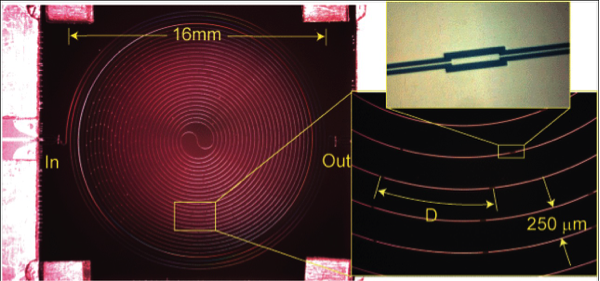
\includegraphics[width=0.45\textwidth]{images/TKIP.png}
%     \end{center}
%     \vspace{-20pt}
% %     \caption{Gamma ray spectrum of $\sim$ 0.4 g of \textsuperscript{239}Pu + \textsuperscript{240}Pu from 40 keV to 220 keV (inset) as measured by the microcalorimeter array developed by \cite{Bennet2012} (blue) and a leading edge HPGe detector (red). Data is magnified in the the 100 keV region. The proposed detector would produce an spectrum competitive with the microcalorimeter array. Image taken from \cite{Bennet2012}. }
% %     \vspace{-10pt}
%   \label{Fig:PuSpectrum}
%  \end{wrapfigure}
%
%
% \ctable[%%%%%%%%%% Lorenz Number
%   cap  =  Temperature & material dependence of Lorenz number,
%   caption = {Temperature and material dependence of Lorenz number used in the Wiedemann-Franz-Lorenz law. Ideally the number should be temperature and material independent. However we observe significant temperature variation. This underscored the necessity to use measured values of thermal conductivity when making heat conduction calculations. Copper is presented by itself due to larger temperature variation in its Lorenz number. },
%   pos = ht!,
%   label   = Fig:Lorenz_Number,
%   figure, botcap,
% ]{ccc}{}{
% 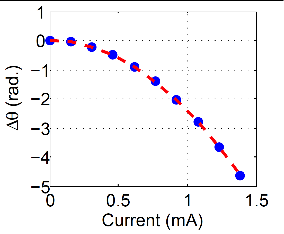
\includegraphics[width=0.24\textwidth]{images/Phase_Response.png}
%  &
% 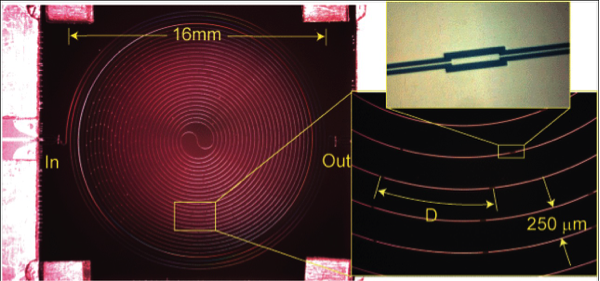
\includegraphics[width=0.48\textwidth]{images/TKIP.png}
% &
% 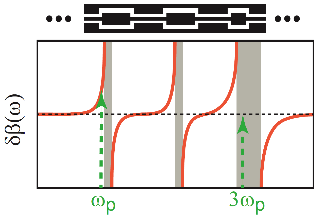
\includegraphics[width=0.24\textwidth]{images/Stop_Bands.png}
% \\
%  }
%
%
% \ctable[%%%%%%%%%% Lorenz Number
%   cap  =  Temperature & material dependence of Lorenz number,
%   caption = {Temperature and material dependence of Lorenz number used in the Wiedemann-Franz-Lorenz law. Ideally the number should be temperature and material independent. However we observe significant temperature variation. This underscored the necessity to use measured values of thermal conductivity when making heat conduction calculations. Copper is presented by itself due to larger temperature variation in its Lorenz number. },
%   pos = ht!,
%   label   = Fig:Lorenz_Number,
%   figure, botcap,
% ]{cc}{}{
% 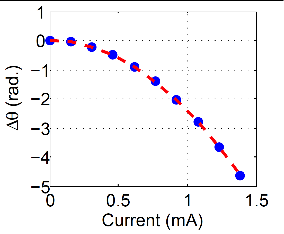
\includegraphics[width=0.48\textwidth]{images/Phase_Response.png}
%  &
% 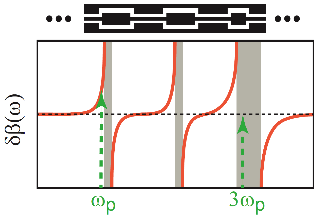
\includegraphics[width=0.48\textwidth]{images/Stop_Bands.png}
% \\
% \multicolumn{2}{c}{
%  \begin{overpic}[width=.96\textwidth]{images/TKIP.png}
%   \put (95,50) {\textcolor{black}{a}}
%  \end{overpic}}
% \\
%  }




  
  


% [Table.~\ref{tab:gammadettechnology}]
% \cite{Bennet2012}

% \begin{table}[htbp]
%   \centering
%   \caption{Comparison of technology between the NIST-LANL microcalorimeter and HPGe ionization detector, representing the most sensitive and most used gamma-ray detectors respectively. $C$ is the combined heat capacity of the TES and the absorber, $F_{fano}$ is the fano factor and other parameters are as defined in Table~\ref{tab:detparams}. `Trans' is the percentage of incident 100 keV gammas that make it through the absorber. Figures listed for the proposed detector represent performance objective achievable on paper.}
%     \begin{tabular}{ccccccc}
%     \toprule
%     Technology & Temp & $\Delta E/E$ & $\Delta E(E)$ & Absorber &Trans & Cts/Sec \\
%     \midrule
%     Planar HPGe & $77 K$ & $3 - 5 \cdot 10^{-3}$ & $\sqrt{F_{fano}\cdot\epsilon_{gap}\cdot E}$ & Sn &$23\% ,\; 5 \, mm $ & $40\cdot 10^{3}$ \\
%     NIST-LANL & $0.1 K$ & $4\cdot 10^{-4}$ & $T \sqrt{k_{B}\cdot C}$ & Ge & $ 63\% ,\; 0.38 \, mm$ & $2.5\cdot 10^{3}$ \\
% 	Proposed & $0.1 K$ & $ \sim 10^{-4}$ & $\sqrt{T_{amp}}$\textsuperscript{See Eq.~\ref{hemtnoise}} & Nb & $ 10^{-6}\% ,\; 5 \,mm$ & $40\cdot  10^{3}$ \\
%     \bottomrule
%     \end{tabular}%
%   \label{tab:gammadettechnology}%
% \end{table}%


% \begin{wrapfigure}{l}{0.74\textwidth} %position can be  r l i or o
%     \vspace{-20pt}
%     \begin{center}
%         \includegraphics[width=0.75\textwidth]{images/Dimensioned_Cross_Section_20140802.png}
%     \end{center}
%     \vspace{-20pt}
%     \caption{Magnified cross section of detector concept utilizing vacuum gap microstrip resonators to sense phonons. A patch of low gap superconductor (e.g. Al or TiN) is located beneath each resonator. Phonons impinging on the patch emanating from within the superconductor absorber break Cooper pairs and change its surface impedance which alters the resonance. Likely dimensions are $w$ = 200 $\mu m$; $t$ = 200 $nm$; $d$ = 3 $\mu m$.}
%     \vspace{-20pt}
%   \label{Fig:PhononsImpinge}
% \end{wrapfigure}











\singlespacing
\footnotesize
\printbibliography 

% \begin{thebibliography}{8}
% \singlespacing
% \footnotesize
% \setlength{\itemsep}{0pt}
% \bibitem{Bennet2012}
%     Bennet D.A., Horansky R. D. 2012. Rev. Sci. Instru. 83:093113
% \bibitem{Zmuidzinas2012}
%     Zmuidzinas, J. 2012. Ann. Rev. Cond. Mat .Phys. 3:169-214
% \bibitem{Vissers2013}
%     Vissers M.R., Gao J., Sandberg M, Duff S.M., Wisbey D.S., Irwin K.D, Pappas D.P. 2013. App. Phys. Lett. 102:232603
% \bibitem{Day2012}
%     Byeong Ho Eom, Day P.K., LeDuc H.G., Zmuidzinas J.,2012. Nature. 8:623-6272013
% \bibitem{Mazin2004}
%     Mazin  B. 2004. Microwave Kinetic Inductance Detectors. PhD Thesis. Cal. Inst. Tech., Pasadena. 179pp.
% \bibitem{Mazin2013} %2024 channel mux
%     Mazin B., Meeker S. R., Strader M. J., Szpryt P., et al. 2013. PASP, 125:1348-1361
% \bibitem{Yates2011} %Aluminum
% 	Yates S. J. C., Baselmans J. J. A., Endo A., et al. 2011. App. Phys. Lett. 99:073505
% %\bibitem{Hubmayr2014} % TiN/Ti
% %	Hubmayr J., Beall J., Becker B., Cho H.-M., et al. 2014 arXiv:1406.4010v1 [astro-ph.IM]
% %\bibitem{McKenney2012}  %non-stoc TiN
% %	McKenney C. M., Leduc H. G.,Swenson L. J., Day P. K., et al. 2012. Proc. of SPIE Vol. 8452:84520S-2
% \bibitem{Hauser1995}
%     Hauser M. 1995. Acoustic waves in crystals: I. Ultrasonic flux Imaging and internal diffraction, II. Imaging Phonons in superconducting niobium. PhD Thesis. U. Illinois at Urbana-Champaign. 131pp.
% \end{thebibliography}


% \paragraph{Outline}
% First we start with a little <  example of the article class, which is an 
% important documentclass. But there would be other documentclasses like 
% book \ref{book}, report \ref{report} and letter \ref{letter} which are 
% described in Section \ref{documentclasses}. Finally, Section 
% \ref{conclusions} gives the conclusions.
% 
% 
% 
% \section{Documentclasses} \label{documentclasses}
% 
% \begin{itemize}
% \item article
% \item book 
% \item report 
% \item letter 
% \end{itemize}
% 
% 
% \begin{enumerate}
% \item article
% \item book 
% \item report 
% \item letter 
% \end{enumerate}
% 
% \begin{description}
% \item[article\label{article}]{Article is \ldots}
% \item[book\label{book}]{The book class \ldots}
% \item[report\label{report}]{Report gives you \ldots}
% \item[letter\label{letter}]{If you want to write a letter.}
% \end{description}







\end{document}

%----
%\section{Introduction}

%\bibliographystyle{plain}
%\bibliography{}
%\end{document}

% Notes:
% Nuclear energy institute: 12.3 % world energy in 2012
% as of May 2014, 30 countries  have 435 power plants, US has 100 w ~1GW capacity
%
% Pu238 for Multi-Mission Radioisotope Thermoelectric Generators (MMRTG, or formerly simply RTGs)
%
% Read more: http://www.universetoday.com/100875/u-s-to-restart-plutonium-production-for-deep-space-exploration/#ixzz38nmVIuRE
